\documentclass[twoside]{book}

% Packages required by doxygen
\usepackage{fixltx2e}
\usepackage{calc}
\usepackage{doxygen}
\usepackage[export]{adjustbox} % also loads graphicx
\usepackage{graphicx}
\usepackage[utf8]{inputenc}
\usepackage{makeidx}
\usepackage{multicol}
\usepackage{multirow}
\PassOptionsToPackage{warn}{textcomp}
\usepackage{textcomp}
\usepackage[nointegrals]{wasysym}
\usepackage[table]{xcolor}

% Font selection
\usepackage[T1]{fontenc}
\usepackage[scaled=.90]{helvet}
\usepackage{courier}
\usepackage{amssymb}
\usepackage{sectsty}
\renewcommand{\familydefault}{\sfdefault}
\allsectionsfont{%
  \fontseries{bc}\selectfont%
  \color{darkgray}%
}
\renewcommand{\DoxyLabelFont}{%
  \fontseries{bc}\selectfont%
  \color{darkgray}%
}
\newcommand{\+}{\discretionary{\mbox{\scriptsize$\hookleftarrow$}}{}{}}

% Page & text layout
\usepackage{geometry}
\geometry{%
  a4paper,%
  top=2.5cm,%
  bottom=2.5cm,%
  left=2.5cm,%
  right=2.5cm%
}
\tolerance=750
\hfuzz=15pt
\hbadness=750
\setlength{\emergencystretch}{15pt}
\setlength{\parindent}{0cm}
\setlength{\parskip}{3ex plus 2ex minus 2ex}
\makeatletter
\renewcommand{\paragraph}{%
  \@startsection{paragraph}{4}{0ex}{-1.0ex}{1.0ex}{%
    \normalfont\normalsize\bfseries\SS@parafont%
  }%
}
\renewcommand{\subparagraph}{%
  \@startsection{subparagraph}{5}{0ex}{-1.0ex}{1.0ex}{%
    \normalfont\normalsize\bfseries\SS@subparafont%
  }%
}
\makeatother

% Headers & footers
\usepackage{fancyhdr}
\pagestyle{fancyplain}
\fancyhead[LE]{\fancyplain{}{\bfseries\thepage}}
\fancyhead[CE]{\fancyplain{}{}}
\fancyhead[RE]{\fancyplain{}{\bfseries\leftmark}}
\fancyhead[LO]{\fancyplain{}{\bfseries\rightmark}}
\fancyhead[CO]{\fancyplain{}{}}
\fancyhead[RO]{\fancyplain{}{\bfseries\thepage}}
\fancyfoot[LE]{\fancyplain{}{}}
\fancyfoot[CE]{\fancyplain{}{}}
\fancyfoot[RE]{\fancyplain{}{\bfseries\scriptsize Generated by Doxygen }}
\fancyfoot[LO]{\fancyplain{}{\bfseries\scriptsize Generated by Doxygen }}
\fancyfoot[CO]{\fancyplain{}{}}
\fancyfoot[RO]{\fancyplain{}{}}
\renewcommand{\footrulewidth}{0.4pt}
\renewcommand{\chaptermark}[1]{%
  \markboth{#1}{}%
}
\renewcommand{\sectionmark}[1]{%
  \markright{\thesection\ #1}%
}

% Indices & bibliography
\usepackage{natbib}
\usepackage[titles]{tocloft}
\setcounter{tocdepth}{3}
\setcounter{secnumdepth}{5}
\makeindex

% Hyperlinks (required, but should be loaded last)
\usepackage{ifpdf}
\ifpdf
  \usepackage[pdftex,pagebackref=true]{hyperref}
\else
  \usepackage[ps2pdf,pagebackref=true]{hyperref}
\fi
\hypersetup{%
  colorlinks=true,%
  linkcolor=blue,%
  citecolor=blue,%
  unicode%
}

% Custom commands
\newcommand{\clearemptydoublepage}{%
  \newpage{\pagestyle{empty}\cleardoublepage}%
}

\usepackage{caption}
\captionsetup{labelsep=space,justification=centering,font={bf},singlelinecheck=off,skip=4pt,position=top}

%===== C O N T E N T S =====

\begin{document}

% Titlepage & ToC
\hypersetup{pageanchor=false,
             bookmarksnumbered=true,
             pdfencoding=unicode
            }
\pagenumbering{roman}
\begin{titlepage}
\vspace*{7cm}
\begin{center}%
{\Large Robot Controller Module \\[1ex]\large 1.\+0 }\\
\vspace*{1cm}
{\large Generated by Doxygen 1.8.11}\\
\end{center}
\end{titlepage}
\clearemptydoublepage
\tableofcontents
\clearemptydoublepage
\pagenumbering{arabic}
\hypersetup{pageanchor=true}

%--- Begin generated contents ---
\chapter{Robot Controller Module}
\label{md_README}
\hypertarget{md_README}{}
\href{https://travis-ci.org/RajPShinde/Robot_Controller_Module}{\tt } \href{https://coveralls.io/github/RajPShinde/Robot_Controller_Module?branch=master}{\tt } \href{https://github.com/RajPShinde/Robot_Controller_Module/blob/master/LICENSE}{\tt } \subsection*{\href{https://github.com/RajPShinde/Robot_Controller_Module/tree/master/docs}{\tt } }

\subsection*{Authors}


\begin{DoxyItemize}
\item {\bfseries Raj Prakash Shinde} -\/ {\itshape Sprint 1-\/ Driver \& Sprint 2-\/ Navigator} -\/ \href{https://github.com/RajPShinde}{\tt Git\+Hub} ~\newline
I am a Masters in Robotics Engineering student at the University of Maryland, College Park. My primary area of interest are Legged Robotics and Automation.
\item {\bfseries Prasheel Renkuntla} -\/ {\itshape Sprint 1-\/ Navigator \& Sprint 2-\/ Driver} -\/ \href{https://github.com/Prasheel24}{\tt Git\+Hub} ~\newline
I am a Master\textquotesingle{}s in Robotics Engineering student at the University of Maryland, College Park. My primary area of interest is in Vision integrated Robot Systems.
\end{DoxyItemize}

\subsection*{Overview}

This is a controller module for a robot that uses an Ackermann Steering Model, This controller is to be implemented in a four wheeled Robot made by A\+C\+ME Robotics.

\paragraph*{Description}

A controller is build for a 4 wheeled robot with an Ackermann steering to navigate through its environment. The controller consist of a P\+ID algorithm which ensures that the velocity converges to the set point, and a Steer Algorithm that helps the robot turn. ~\newline
The P\+ID Algorithm is a control loop mechanism that calculates the error and applies correction through proportional, integral and derivative gains. The Steer Algorithm is developed to turn the robot, which is done by calculating the length of an arc inscribed between the current robot heading and target heading, the length when divided by the robot velocity gives the time for which the wheels need to be kept at angles given by Ackermann steering Model. ~\newline
The input to the controller will be provided by the perception model developed by the A\+C\+ME Robotics. ~\newline
The Demonstration of the controller will be given by plotting a graph that shows convergence of velocity \& Heading angle to the targets with respect to time.

\paragraph*{Features}


\begin{DoxyItemize}
\item Velocity control during turning.
\item Protection against Skidding, by limiting velocity during turning.
\item Protection agains over volting the Motors.
\end{DoxyItemize}

\paragraph*{Application}


\begin{DoxyItemize}
\item Mobile Wheeled Robots
\end{DoxyItemize}

\subsection*{Sprint Planning and Discussion}

Sprint-\/ \href{https://docs.google.com/document/d/1w6U49tyKj9MFhaVziZ5MEGcaylmxSBOyGzClIz9lFA8/edit?usp=sharing}{\tt https\+://docs.\+google.\+com/document/d/1w6\+U49ty\+Kj9\+M\+Fha\+Vzi\+Z5\+M\+E\+Gcaylmx\+S\+B\+Oy\+Gz\+Cl\+Iz9l\+F\+A8/edit?usp=sharing}

\subsection*{Agile Iterative Process Log}

Log-\/ \href{https://docs.google.com/spreadsheets/d/1LFQMKbuGeusgmI7IMbjiw-RJrt9jNgej0F8SvvfyJjY/edit?usp=sharing}{\tt https\+://docs.\+google.\+com/spreadsheets/d/1\+L\+F\+Q\+M\+Kbu\+Geusgm\+I7\+I\+Mbjiw-\/\+R\+Jrt9j\+Ngej0\+F8\+Svvfy\+Jj\+Y/edit?usp=sharing}

\subsection*{Dependencies}


\begin{DoxyEnumerate}
\item C++ 11/14/17
\item gnuplot ~\newline
Install gnuplot 
\begin{DoxyCode}
1 sudo apt-get install gnuplot
\end{DoxyCode}

\item boost ~\newline
Install boost 
\begin{DoxyCode}
1 sudo apt-get install libboost-all-dev
\end{DoxyCode}

\end{DoxyEnumerate}

\#\# Build 
\begin{DoxyCode}
1 git clone --recursive https://github.com/RajPShinde/Robot\_Controller\_Module.git
2 cd <path to repository>
3 mkdir build
4 cd build
5 cmake ..
6 make
\end{DoxyCode}
 \subsection*{Run}

\#\#\#\# Run Program 
\begin{DoxyCode}
1 ./app/shell-app
\end{DoxyCode}
 \#\#\#\# Run Test 
\begin{DoxyCode}
1 ./test/cpp-test
\end{DoxyCode}
 \subsection*{Demo}

Run the program. Once the velocity and heading converge to the target then graphs will be displayed as below. Also, converged values will be shown in the terminal.

\subparagraph*{Heading Convergence}

 

\subparagraph*{Velocity Convergence}

 

\subparagraph*{Terminal Output}

 

\subsection*{Bugs}

None

\subsection*{References}


\begin{DoxyItemize}
\item Ackermann Steering-\/ \href{https://www.sciencedirect.com/topics/engineering/ackermann}{\tt https\+://www.\+sciencedirect.\+com/topics/engineering/ackermann}
\item P\+ID Controller-\/ \href{https://en.wikipedia.org/wiki/PID_controller}{\tt https\+://en.\+wikipedia.\+org/wiki/\+P\+I\+D\+\_\+controller}
\item gnuplot-\/ \href{http://stahlke.org/dan/gnuplot-iostream/}{\tt http\+://stahlke.\+org/dan/gnuplot-\/iostream/} 
\end{DoxyItemize}
\chapter{Hierarchical Index}
\section{Class Hierarchy}
This inheritance list is sorted roughly, but not completely, alphabetically\+:\begin{DoxyCompactList}
\item \contentsline{section}{Steer\+Algorithm}{\pageref{class_steer_algorithm}}{}
\begin{DoxyCompactList}
\item \contentsline{section}{Navigation}{\pageref{class_navigation}}{}
\end{DoxyCompactList}
\end{DoxyCompactList}

\chapter{Class Index}
\section{Class List}
Here are the classes, structs, unions and interfaces with brief descriptions\+:\begin{DoxyCompactList}
\item\contentsline{section}{\hyperlink{class_navigation}{Navigation} \\*Class \hyperlink{class_navigation}{Navigation} Contains the methods of Pid Algorithm }{\pageref{class_navigation}}{}
\item\contentsline{section}{\hyperlink{class_steer_algorithm}{Steer\+Algorithm} \\*Class \hyperlink{class_steer_algorithm}{Steer\+Algorithm} contains the methods of the Steering Algorithm }{\pageref{class_steer_algorithm}}{}
\end{DoxyCompactList}

\chapter{File Index}
\section{File List}
Here is a list of all documented files with brief descriptions\+:\begin{DoxyCompactList}
\item\contentsline{section}{app/\hyperlink{_navigation_8cpp}{Navigation.\+cpp} \\*Mid Term Project }{\pageref{_navigation_8cpp}}{}
\item\contentsline{section}{app/\hyperlink{_steer_algorithm_8cpp}{Steer\+Algorithm.\+cpp} \\*Mid Term Project }{\pageref{_steer_algorithm_8cpp}}{}
\item\contentsline{section}{include/\hyperlink{_navigation_8hpp}{Navigation.\+hpp} \\*Mid Term Project }{\pageref{_navigation_8hpp}}{}
\item\contentsline{section}{include/\hyperlink{_steer_algorithm_8hpp}{Steer\+Algorithm.\+hpp} \\*Mid Term Project }{\pageref{_steer_algorithm_8hpp}}{}
\item\contentsline{section}{test/\hyperlink{test_navigation_8cpp}{test\+Navigation.\+cpp} \\*Mid Term Project }{\pageref{test_navigation_8cpp}}{}
\item\contentsline{section}{test/\hyperlink{test_steer_algorithm_8cpp}{test\+Steer\+Algorithm.\+cpp} \\*Mid Term Project }{\pageref{test_steer_algorithm_8cpp}}{}
\end{DoxyCompactList}

\chapter{Class Documentation}
\hypertarget{class_navigation}{}\section{Navigation Class Reference}
\label{class_navigation}\index{Navigation@{Navigation}}


Class \hyperlink{class_navigation}{Navigation} Contains the methods of Pid Algorithm.  




{\ttfamily \#include $<$Navigation.\+hpp$>$}



Inheritance diagram for Navigation\+:
\nopagebreak
\begin{figure}[H]
\begin{center}
\leavevmode
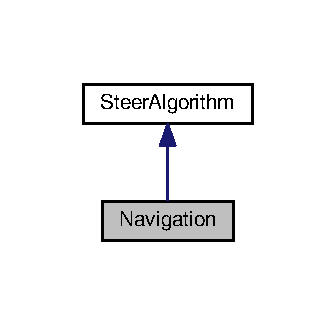
\includegraphics[width=161pt]{class_navigation__inherit__graph}
\end{center}
\end{figure}


Collaboration diagram for Navigation\+:
\nopagebreak
\begin{figure}[H]
\begin{center}
\leavevmode
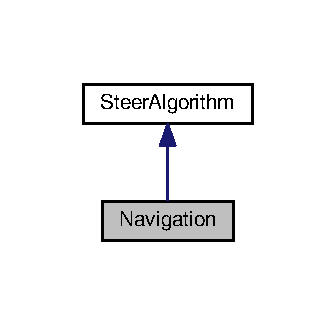
\includegraphics[width=161pt]{class_navigation__coll__graph}
\end{center}
\end{figure}
\subsection*{Public Member Functions}
\begin{DoxyCompactItemize}
\item 
\hyperlink{class_navigation_a81fdffdefe46340da5fa6c570066b42b}{Navigation} ()\hypertarget{class_navigation_a81fdffdefe46340da5fa6c570066b42b}{}\label{class_navigation_a81fdffdefe46340da5fa6c570066b42b}

\begin{DoxyCompactList}\small\item\em Constructor of class \hyperlink{class_navigation}{Navigation}. \end{DoxyCompactList}\item 
\hyperlink{class_navigation_addd4022d716df48f4e55a1db69361ba7}{$\sim$\+Navigation} ()\hypertarget{class_navigation_addd4022d716df48f4e55a1db69361ba7}{}\label{class_navigation_addd4022d716df48f4e55a1db69361ba7}

\begin{DoxyCompactList}\small\item\em Destructor of class \hyperlink{class_navigation}{Navigation}. \end{DoxyCompactList}\item 
double \hyperlink{class_navigation_a0eb1833ccc91d6fd5822938797686708}{calculate} (double current\+Velocity, double set\+Point, int flag)
\begin{DoxyCompactList}\small\item\em Function to calculate new velocity with a P\+ID Algorithm using kp, ki \& kd. \end{DoxyCompactList}\item 
double \hyperlink{class_navigation_ab1469d74f4838a9d32a8647d22701f9f}{get\+Kp\+\_\+} ()
\begin{DoxyCompactList}\small\item\em Function to get kp\+\_\+. \end{DoxyCompactList}\item 
double \hyperlink{class_navigation_a1a84392d6cce3f60df452ab482b5647c}{get\+Ki\+\_\+} ()
\begin{DoxyCompactList}\small\item\em Function to get ki\+\_\+. \end{DoxyCompactList}\item 
double \hyperlink{class_navigation_ac6441bb601483166ef7a8081b76f634d}{get\+Kd\+\_\+} ()
\begin{DoxyCompactList}\small\item\em Function to get kd\+\_\+. \end{DoxyCompactList}\item 
bool \hyperlink{class_navigation_a6dd95f46ff4ecc69895452a1879c30af}{set\+Kp\+\_\+} (double kp)
\begin{DoxyCompactList}\small\item\em Function to set kp\+\_\+. \end{DoxyCompactList}\item 
bool \hyperlink{class_navigation_a539d10206ceb162171e39c36e8aa8f0f}{set\+Ki\+\_\+} (double ki)
\begin{DoxyCompactList}\small\item\em Function to set ki\+\_\+. \end{DoxyCompactList}\item 
bool \hyperlink{class_navigation_a4986e4357d9707ddf92cf8f559ef3dce}{set\+Kd\+\_\+} (double kd)
\begin{DoxyCompactList}\small\item\em Function to set kd\+\_\+. \end{DoxyCompactList}\end{DoxyCompactItemize}
\subsection*{Public Attributes}
\begin{DoxyCompactItemize}
\item 
bool {\bfseries motor\+Direction} = true\hypertarget{class_navigation_ad7d7a5d5d1abe99e6b0f31ddb4794252}{}\label{class_navigation_ad7d7a5d5d1abe99e6b0f31ddb4794252}

\end{DoxyCompactItemize}


\subsection{Detailed Description}
Class \hyperlink{class_navigation}{Navigation} Contains the methods of Pid Algorithm. 

\subsection{Member Function Documentation}
\index{Navigation@{Navigation}!calculate@{calculate}}
\index{calculate@{calculate}!Navigation@{Navigation}}
\subsubsection[{\texorpdfstring{calculate(double current\+Velocity, double set\+Point, int flag)}{calculate(double currentVelocity, double setPoint, int flag)}}]{\setlength{\rightskip}{0pt plus 5cm}double Navigation\+::calculate (
\begin{DoxyParamCaption}
\item[{double}]{current\+Velocity, }
\item[{double}]{set\+Point, }
\item[{int}]{flag}
\end{DoxyParamCaption}
)}\hypertarget{class_navigation_a0eb1833ccc91d6fd5822938797686708}{}\label{class_navigation_a0eb1833ccc91d6fd5822938797686708}


Function to calculate new velocity with a P\+ID Algorithm using kp, ki \& kd. 


\begin{DoxyParams}{Parameters}
{\em double} & current\+Velocity, current velocity of robot \\
\hline
{\em double} & set\+Point, Target Velocity \\
\hline
{\em int} & flag, to enable while \\
\hline
\end{DoxyParams}
\begin{DoxyReturn}{Returns}
double ne\+Velocity 
\end{DoxyReturn}
\index{Navigation@{Navigation}!get\+Kd\+\_\+@{get\+Kd\+\_\+}}
\index{get\+Kd\+\_\+@{get\+Kd\+\_\+}!Navigation@{Navigation}}
\subsubsection[{\texorpdfstring{get\+Kd\+\_\+()}{getKd_()}}]{\setlength{\rightskip}{0pt plus 5cm}double Navigation\+::get\+Kd\+\_\+ (
\begin{DoxyParamCaption}
{}
\end{DoxyParamCaption}
)}\hypertarget{class_navigation_ac6441bb601483166ef7a8081b76f634d}{}\label{class_navigation_ac6441bb601483166ef7a8081b76f634d}


Function to get kd\+\_\+. 


\begin{DoxyParams}{Parameters}
{\em none} & \\
\hline
\end{DoxyParams}
\begin{DoxyReturn}{Returns}
double 
\end{DoxyReturn}
\index{Navigation@{Navigation}!get\+Ki\+\_\+@{get\+Ki\+\_\+}}
\index{get\+Ki\+\_\+@{get\+Ki\+\_\+}!Navigation@{Navigation}}
\subsubsection[{\texorpdfstring{get\+Ki\+\_\+()}{getKi_()}}]{\setlength{\rightskip}{0pt plus 5cm}double Navigation\+::get\+Ki\+\_\+ (
\begin{DoxyParamCaption}
{}
\end{DoxyParamCaption}
)}\hypertarget{class_navigation_a1a84392d6cce3f60df452ab482b5647c}{}\label{class_navigation_a1a84392d6cce3f60df452ab482b5647c}


Function to get ki\+\_\+. 


\begin{DoxyParams}{Parameters}
{\em none} & \\
\hline
\end{DoxyParams}
\begin{DoxyReturn}{Returns}
double 
\end{DoxyReturn}
\index{Navigation@{Navigation}!get\+Kp\+\_\+@{get\+Kp\+\_\+}}
\index{get\+Kp\+\_\+@{get\+Kp\+\_\+}!Navigation@{Navigation}}
\subsubsection[{\texorpdfstring{get\+Kp\+\_\+()}{getKp_()}}]{\setlength{\rightskip}{0pt plus 5cm}double Navigation\+::get\+Kp\+\_\+ (
\begin{DoxyParamCaption}
{}
\end{DoxyParamCaption}
)}\hypertarget{class_navigation_ab1469d74f4838a9d32a8647d22701f9f}{}\label{class_navigation_ab1469d74f4838a9d32a8647d22701f9f}


Function to get kp\+\_\+. 


\begin{DoxyParams}{Parameters}
{\em none} & \\
\hline
\end{DoxyParams}
\begin{DoxyReturn}{Returns}
double 
\end{DoxyReturn}
\index{Navigation@{Navigation}!set\+Kd\+\_\+@{set\+Kd\+\_\+}}
\index{set\+Kd\+\_\+@{set\+Kd\+\_\+}!Navigation@{Navigation}}
\subsubsection[{\texorpdfstring{set\+Kd\+\_\+(double kd)}{setKd_(double kd)}}]{\setlength{\rightskip}{0pt plus 5cm}bool Navigation\+::set\+Kd\+\_\+ (
\begin{DoxyParamCaption}
\item[{double}]{kd}
\end{DoxyParamCaption}
)}\hypertarget{class_navigation_a4986e4357d9707ddf92cf8f559ef3dce}{}\label{class_navigation_a4986e4357d9707ddf92cf8f559ef3dce}


Function to set kd\+\_\+. 


\begin{DoxyParams}{Parameters}
{\em double} & kd \\
\hline
\end{DoxyParams}
\begin{DoxyReturn}{Returns}
boolean true 
\end{DoxyReturn}
\index{Navigation@{Navigation}!set\+Ki\+\_\+@{set\+Ki\+\_\+}}
\index{set\+Ki\+\_\+@{set\+Ki\+\_\+}!Navigation@{Navigation}}
\subsubsection[{\texorpdfstring{set\+Ki\+\_\+(double ki)}{setKi_(double ki)}}]{\setlength{\rightskip}{0pt plus 5cm}bool Navigation\+::set\+Ki\+\_\+ (
\begin{DoxyParamCaption}
\item[{double}]{ki}
\end{DoxyParamCaption}
)}\hypertarget{class_navigation_a539d10206ceb162171e39c36e8aa8f0f}{}\label{class_navigation_a539d10206ceb162171e39c36e8aa8f0f}


Function to set ki\+\_\+. 


\begin{DoxyParams}{Parameters}
{\em double} & ki \\
\hline
\end{DoxyParams}
\begin{DoxyReturn}{Returns}
boolean true 
\end{DoxyReturn}
\index{Navigation@{Navigation}!set\+Kp\+\_\+@{set\+Kp\+\_\+}}
\index{set\+Kp\+\_\+@{set\+Kp\+\_\+}!Navigation@{Navigation}}
\subsubsection[{\texorpdfstring{set\+Kp\+\_\+(double kp)}{setKp_(double kp)}}]{\setlength{\rightskip}{0pt plus 5cm}bool Navigation\+::set\+Kp\+\_\+ (
\begin{DoxyParamCaption}
\item[{double}]{kp}
\end{DoxyParamCaption}
)}\hypertarget{class_navigation_a6dd95f46ff4ecc69895452a1879c30af}{}\label{class_navigation_a6dd95f46ff4ecc69895452a1879c30af}


Function to set kp\+\_\+. 


\begin{DoxyParams}{Parameters}
{\em double} & kp \\
\hline
\end{DoxyParams}
\begin{DoxyReturn}{Returns}
boolean true 
\end{DoxyReturn}


The documentation for this class was generated from the following files\+:\begin{DoxyCompactItemize}
\item 
include/\hyperlink{_navigation_8hpp}{Navigation.\+hpp}\item 
app/\hyperlink{_navigation_8cpp}{Navigation.\+cpp}\end{DoxyCompactItemize}

\hypertarget{class_steer_algorithm}{}\section{Steer\+Algorithm Class Reference}
\label{class_steer_algorithm}\index{Steer\+Algorithm@{Steer\+Algorithm}}


Class \hyperlink{class_steer_algorithm}{Steer\+Algorithm} contains the methods of the Steering Algorithm.  




{\ttfamily \#include $<$Steer\+Algorithm.\+hpp$>$}



Inheritance diagram for Steer\+Algorithm\+:
\nopagebreak
\begin{figure}[H]
\begin{center}
\leavevmode
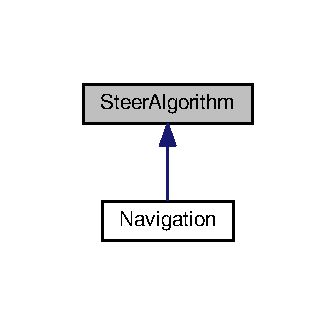
\includegraphics[width=161pt]{class_steer_algorithm__inherit__graph}
\end{center}
\end{figure}
\subsection*{Public Member Functions}
\begin{DoxyCompactItemize}
\item 
\hyperlink{class_steer_algorithm_af64dd94816ab9d00d85227a42b26a3e8}{Steer\+Algorithm} ()\hypertarget{class_steer_algorithm_af64dd94816ab9d00d85227a42b26a3e8}{}\label{class_steer_algorithm_af64dd94816ab9d00d85227a42b26a3e8}

\begin{DoxyCompactList}\small\item\em Constructor of class \hyperlink{class_steer_algorithm}{Steer\+Algorithm}. \end{DoxyCompactList}\item 
\hyperlink{class_steer_algorithm_a37dd2ef0ed856582aaacc103a6cd6700}{$\sim$\+Steer\+Algorithm} ()\hypertarget{class_steer_algorithm_a37dd2ef0ed856582aaacc103a6cd6700}{}\label{class_steer_algorithm_a37dd2ef0ed856582aaacc103a6cd6700}

\begin{DoxyCompactList}\small\item\em Destructor of class \hyperlink{class_steer_algorithm}{Steer\+Algorithm}. \end{DoxyCompactList}\item 
double \hyperlink{class_steer_algorithm_a06a7dd049280fab40d1b54c912daf399}{get\+Corr\+Radius\+\_\+} ()
\begin{DoxyCompactList}\small\item\em Function to get corresponding radius in meters. \end{DoxyCompactList}\item 
bool \hyperlink{class_steer_algorithm_a93cf1fc7d06376ddeaa4e81f2b0a22cc}{set\+Corr\+Radius\+\_\+} (double r)
\begin{DoxyCompactList}\small\item\em Function to set corresponding radius in meters. \end{DoxyCompactList}\item 
double \hyperlink{class_steer_algorithm_a17ff78af17e900f752237d274bcf751d}{arc\+Length} (double diff\+Angle, double corr\+Radius)
\begin{DoxyCompactList}\small\item\em Function to calculate the length of arc in meters to be traced in order to head in target direction. \end{DoxyCompactList}\item 
double \hyperlink{class_steer_algorithm_a6067af69593713f561890ae8ad23f5ff}{change\+Wheel\+Angles} (double corr\+Radius, double shaft\+Length, double shaft\+Distance)
\begin{DoxyCompactList}\small\item\em Function to calculate the angles in degrees for left and right wheels as per ackermann model, and then feed them to corresponding servos. \end{DoxyCompactList}\item 
bool \hyperlink{class_steer_algorithm_ab251b6fd1f88fb7a526b0d55cd12625b}{reset\+Wheel} ()
\begin{DoxyCompactList}\small\item\em Function to set wheel angles to 0. \end{DoxyCompactList}\item 
double \hyperlink{class_steer_algorithm_aefdb433f65c47bf6e0d6af5de98c8f5a}{turn\+Time} (double arclength, double new\+Velocity)
\begin{DoxyCompactList}\small\item\em Function to calculate time in seconds required to turn or keep wheels at the an angle. \end{DoxyCompactList}\end{DoxyCompactItemize}
\subsection*{Public Attributes}
\begin{DoxyCompactItemize}
\item 
const double {\bfseries shaft\+Length} = 4\hypertarget{class_steer_algorithm_a9d5bc20acba39f0e53c3d0f6fc280433}{}\label{class_steer_algorithm_a9d5bc20acba39f0e53c3d0f6fc280433}

\item 
const double {\bfseries shaft\+Distance} = 8\hypertarget{class_steer_algorithm_a38bc87552a30e8eda8f647cf341c9657}{}\label{class_steer_algorithm_a38bc87552a30e8eda8f647cf341c9657}

\item 
const double {\bfseries max\+Turn\+Velocity} = 20\hypertarget{class_steer_algorithm_acfce52839329f0ebb316f633494466e1}{}\label{class_steer_algorithm_acfce52839329f0ebb316f633494466e1}

\item 
double {\bfseries heading}\hypertarget{class_steer_algorithm_ada73b1f087245af5cda5d1d6b9be7d31}{}\label{class_steer_algorithm_ada73b1f087245af5cda5d1d6b9be7d31}

\item 
double {\bfseries target\+Heading}\hypertarget{class_steer_algorithm_a071efeb53e86ee949940b0ab10986044}{}\label{class_steer_algorithm_a071efeb53e86ee949940b0ab10986044}

\item 
int {\bfseries dir}\hypertarget{class_steer_algorithm_af6ad5604b62eec22cc2d385c7683d019}{}\label{class_steer_algorithm_af6ad5604b62eec22cc2d385c7683d019}

\end{DoxyCompactItemize}


\subsection{Detailed Description}
Class \hyperlink{class_steer_algorithm}{Steer\+Algorithm} contains the methods of the Steering Algorithm. 

\subsection{Member Function Documentation}
\index{Steer\+Algorithm@{Steer\+Algorithm}!arc\+Length@{arc\+Length}}
\index{arc\+Length@{arc\+Length}!Steer\+Algorithm@{Steer\+Algorithm}}
\subsubsection[{\texorpdfstring{arc\+Length(double diff\+Angle, double corr\+Radius)}{arcLength(double diffAngle, double corrRadius)}}]{\setlength{\rightskip}{0pt plus 5cm}double Steer\+Algorithm\+::arc\+Length (
\begin{DoxyParamCaption}
\item[{double}]{diff\+Angle, }
\item[{double}]{corr\+Radius}
\end{DoxyParamCaption}
)}\hypertarget{class_steer_algorithm_a17ff78af17e900f752237d274bcf751d}{}\label{class_steer_algorithm_a17ff78af17e900f752237d274bcf751d}


Function to calculate the length of arc in meters to be traced in order to head in target direction. 


\begin{DoxyParams}{Parameters}
{\em double} & diff\+Angle, difference in current and target heading \\
\hline
{\em double} & corr\+Radius, corresponding radius \\
\hline
\end{DoxyParams}
\begin{DoxyReturn}{Returns}
double arclength 
\end{DoxyReturn}
\index{Steer\+Algorithm@{Steer\+Algorithm}!change\+Wheel\+Angles@{change\+Wheel\+Angles}}
\index{change\+Wheel\+Angles@{change\+Wheel\+Angles}!Steer\+Algorithm@{Steer\+Algorithm}}
\subsubsection[{\texorpdfstring{change\+Wheel\+Angles(double corr\+Radius, double shaft\+Length, double shaft\+Distance)}{changeWheelAngles(double corrRadius, double shaftLength, double shaftDistance)}}]{\setlength{\rightskip}{0pt plus 5cm}double Steer\+Algorithm\+::change\+Wheel\+Angles (
\begin{DoxyParamCaption}
\item[{double}]{corr\+Radius, }
\item[{double}]{shaft\+Length, }
\item[{double}]{shaft\+Distance}
\end{DoxyParamCaption}
)}\hypertarget{class_steer_algorithm_a6067af69593713f561890ae8ad23f5ff}{}\label{class_steer_algorithm_a6067af69593713f561890ae8ad23f5ff}


Function to calculate the angles in degrees for left and right wheels as per ackermann model, and then feed them to corresponding servos. 


\begin{DoxyParams}{Parameters}
{\em double} & corr\+Radius, corresponding radius \\
\hline
{\em double} & shaft\+Length, length between wheels \\
\hline
{\em double} & shaf\+Distance, distance between rear and front shaft \\
\hline
\end{DoxyParams}
\begin{DoxyReturn}{Returns}
double max\+Wheel\+Angle 
\end{DoxyReturn}
\index{Steer\+Algorithm@{Steer\+Algorithm}!get\+Corr\+Radius\+\_\+@{get\+Corr\+Radius\+\_\+}}
\index{get\+Corr\+Radius\+\_\+@{get\+Corr\+Radius\+\_\+}!Steer\+Algorithm@{Steer\+Algorithm}}
\subsubsection[{\texorpdfstring{get\+Corr\+Radius\+\_\+()}{getCorrRadius_()}}]{\setlength{\rightskip}{0pt plus 5cm}double Steer\+Algorithm\+::get\+Corr\+Radius\+\_\+ (
\begin{DoxyParamCaption}
{}
\end{DoxyParamCaption}
)}\hypertarget{class_steer_algorithm_a06a7dd049280fab40d1b54c912daf399}{}\label{class_steer_algorithm_a06a7dd049280fab40d1b54c912daf399}


Function to get corresponding radius in meters. 


\begin{DoxyParams}{Parameters}
{\em none} & \\
\hline
\end{DoxyParams}
\begin{DoxyReturn}{Returns}
double corresponding radius 
\end{DoxyReturn}
\index{Steer\+Algorithm@{Steer\+Algorithm}!reset\+Wheel@{reset\+Wheel}}
\index{reset\+Wheel@{reset\+Wheel}!Steer\+Algorithm@{Steer\+Algorithm}}
\subsubsection[{\texorpdfstring{reset\+Wheel()}{resetWheel()}}]{\setlength{\rightskip}{0pt plus 5cm}bool Steer\+Algorithm\+::reset\+Wheel (
\begin{DoxyParamCaption}
{}
\end{DoxyParamCaption}
)}\hypertarget{class_steer_algorithm_ab251b6fd1f88fb7a526b0d55cd12625b}{}\label{class_steer_algorithm_ab251b6fd1f88fb7a526b0d55cd12625b}


Function to set wheel angles to 0. 


\begin{DoxyParams}{Parameters}
{\em none} & \\
\hline
\end{DoxyParams}
\begin{DoxyReturn}{Returns}
bool true 
\end{DoxyReturn}
\index{Steer\+Algorithm@{Steer\+Algorithm}!set\+Corr\+Radius\+\_\+@{set\+Corr\+Radius\+\_\+}}
\index{set\+Corr\+Radius\+\_\+@{set\+Corr\+Radius\+\_\+}!Steer\+Algorithm@{Steer\+Algorithm}}
\subsubsection[{\texorpdfstring{set\+Corr\+Radius\+\_\+(double r)}{setCorrRadius_(double r)}}]{\setlength{\rightskip}{0pt plus 5cm}bool Steer\+Algorithm\+::set\+Corr\+Radius\+\_\+ (
\begin{DoxyParamCaption}
\item[{double}]{r}
\end{DoxyParamCaption}
)}\hypertarget{class_steer_algorithm_a93cf1fc7d06376ddeaa4e81f2b0a22cc}{}\label{class_steer_algorithm_a93cf1fc7d06376ddeaa4e81f2b0a22cc}


Function to set corresponding radius in meters. 


\begin{DoxyParams}{Parameters}
{\em double} & radius \\
\hline
\end{DoxyParams}
\begin{DoxyReturn}{Returns}
bool true 
\end{DoxyReturn}
\index{Steer\+Algorithm@{Steer\+Algorithm}!turn\+Time@{turn\+Time}}
\index{turn\+Time@{turn\+Time}!Steer\+Algorithm@{Steer\+Algorithm}}
\subsubsection[{\texorpdfstring{turn\+Time(double arclength, double new\+Velocity)}{turnTime(double arclength, double newVelocity)}}]{\setlength{\rightskip}{0pt plus 5cm}double Steer\+Algorithm\+::turn\+Time (
\begin{DoxyParamCaption}
\item[{double}]{arclength, }
\item[{double}]{new\+Velocity}
\end{DoxyParamCaption}
)}\hypertarget{class_steer_algorithm_aefdb433f65c47bf6e0d6af5de98c8f5a}{}\label{class_steer_algorithm_aefdb433f65c47bf6e0d6af5de98c8f5a}


Function to calculate time in seconds required to turn or keep wheels at the an angle. 


\begin{DoxyParams}{Parameters}
{\em double} & arc\+Length, length of arc to be traced \\
\hline
{\em double} & new\+Velocity, velocity \\
\hline
\end{DoxyParams}
\begin{DoxyReturn}{Returns}
double time 
\end{DoxyReturn}


The documentation for this class was generated from the following files\+:\begin{DoxyCompactItemize}
\item 
include/\hyperlink{_steer_algorithm_8hpp}{Steer\+Algorithm.\+hpp}\item 
app/\hyperlink{_steer_algorithm_8cpp}{Steer\+Algorithm.\+cpp}\end{DoxyCompactItemize}

\chapter{File Documentation}
\hypertarget{_navigation_8cpp}{}\section{app/\+Navigation.cpp File Reference}
\label{_navigation_8cpp}\index{app/\+Navigation.\+cpp@{app/\+Navigation.\+cpp}}


Mid Term Project.  


{\ttfamily \#include $<$time.\+h$>$}\\*
{\ttfamily \#include $<$gnuplot-\/iostream.\+h$>$}\\*
{\ttfamily \#include $<$iostream$>$}\\*
{\ttfamily \#include $<$fstream$>$}\\*
{\ttfamily \#include $<$vector$>$}\\*
{\ttfamily \#include \char`\"{}Navigation.\+hpp\char`\"{}}\\*
{\ttfamily \#include \char`\"{}Steer\+Algorithm.\+hpp\char`\"{}}\\*
Include dependency graph for Navigation.\+cpp\+:
\nopagebreak
\begin{figure}[H]
\begin{center}
\leavevmode
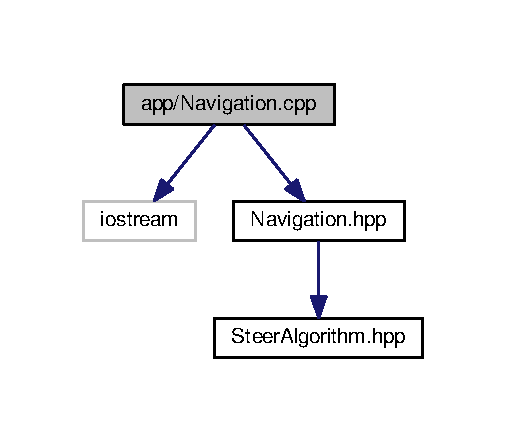
\includegraphics[width=350pt]{_navigation_8cpp__incl}
\end{center}
\end{figure}


\subsection{Detailed Description}
Mid Term Project. 

\begin{DoxyCopyright}{Copyright}
M\+IT License, Copyright © 2019 Raj Shinde
\end{DoxyCopyright}
\begin{DoxyAuthor}{Author}
Sprint-\/1 Raj Shinde-\/ driver and Prasheel Renkuntla-\/ navigator 

Sprint-\/2 Prasheel Renkuntla-\/ driver and Raj Shinde-\/ navigator 
\end{DoxyAuthor}
\begin{DoxyDate}{Date}
10/10/2019 
\end{DoxyDate}
\begin{DoxyVersion}{Version}
6.\+0 
\end{DoxyVersion}
\hypertarget{_steer_algorithm_8cpp_Implements}{}\subsection{Ackermann on P\+I\+D control}\label{_steer_algorithm_8cpp_Implements}

\hypertarget{_steer_algorithm_8cpp}{}\section{app/\+Steer\+Algorithm.cpp File Reference}
\label{_steer_algorithm_8cpp}\index{app/\+Steer\+Algorithm.\+cpp@{app/\+Steer\+Algorithm.\+cpp}}


Mid Term Project.  


{\ttfamily \#include $<$iostream$>$}\\*
{\ttfamily \#include $<$cmath$>$}\\*
{\ttfamily \#include \char`\"{}Steer\+Algorithm.\+hpp\char`\"{}}\\*
Include dependency graph for Steer\+Algorithm.\+cpp\+:
\nopagebreak
\begin{figure}[H]
\begin{center}
\leavevmode
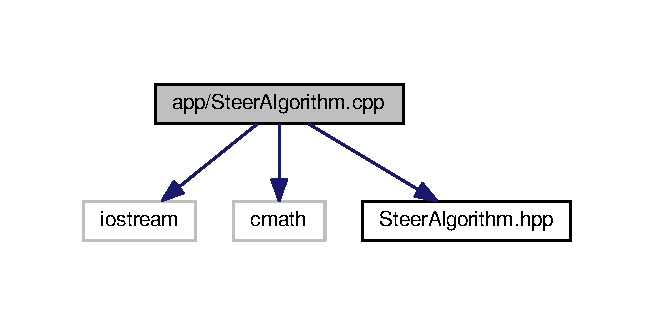
\includegraphics[width=314pt]{_steer_algorithm_8cpp__incl}
\end{center}
\end{figure}


\subsection{Detailed Description}
Mid Term Project. 

\begin{DoxyCopyright}{Copyright}
M\+IT License, Copyright © 2019 Raj Shinde
\end{DoxyCopyright}
\begin{DoxyAuthor}{Author}
Sprint-\/1 Raj Shinde-\/ driver and Prasheel Renkuntla-\/ navigator 

Sprint-\/2 Prasheel Renkuntla-\/ driver and Raj Shinde-\/ navigator 
\end{DoxyAuthor}
\begin{DoxyDate}{Date}
10/10/2019 
\end{DoxyDate}
\begin{DoxyVersion}{Version}
6.\+0 
\end{DoxyVersion}
\hypertarget{_steer_algorithm_8cpp_Implements}{}\subsection{Ackermann on P\+I\+D control}\label{_steer_algorithm_8cpp_Implements}

\hypertarget{_navigation_8hpp}{}\section{include/\+Navigation.hpp File Reference}
\label{_navigation_8hpp}\index{include/\+Navigation.\+hpp@{include/\+Navigation.\+hpp}}


Mid Term Project.  


{\ttfamily \#include \char`\"{}Steer\+Algorithm.\+hpp\char`\"{}}\\*
{\ttfamily \#include $<$vector$>$}\\*
\subsection*{Classes}
\begin{DoxyCompactItemize}
\item 
class \hyperlink{class_navigation}{Navigation}
\begin{DoxyCompactList}\small\item\em Class \hyperlink{class_navigation}{Navigation} Contains the methods of Pid Algorithm. \end{DoxyCompactList}\end{DoxyCompactItemize}


\subsection{Detailed Description}
Mid Term Project. 

\begin{DoxyCopyright}{Copyright}
M\+IT License, Copyright © 2019 Raj Shinde
\end{DoxyCopyright}
\begin{DoxyAuthor}{Author}
Sprint-\/1 Raj Shinde-\/ driver and Prasheel Renkuntla-\/ navigator 

Sprint-\/2 Prasheel Renkuntla-\/ driver and Raj Shinde-\/ navigator 
\end{DoxyAuthor}
\begin{DoxyDate}{Date}
10/10/2019 
\end{DoxyDate}
\begin{DoxyVersion}{Version}
6.\+0 
\end{DoxyVersion}
\hypertarget{_navigation_8hpp_Header}{}\subsection{file for Navigation through P\+I\+D control}\label{_navigation_8hpp_Header}

\hypertarget{_steer_algorithm_8hpp}{}\section{include/\+Steer\+Algorithm.hpp File Reference}
\label{_steer_algorithm_8hpp}\index{include/\+Steer\+Algorithm.\+hpp@{include/\+Steer\+Algorithm.\+hpp}}


Mid Term Project.  


This graph shows which files directly or indirectly include this file\+:
\nopagebreak
\begin{figure}[H]
\begin{center}
\leavevmode
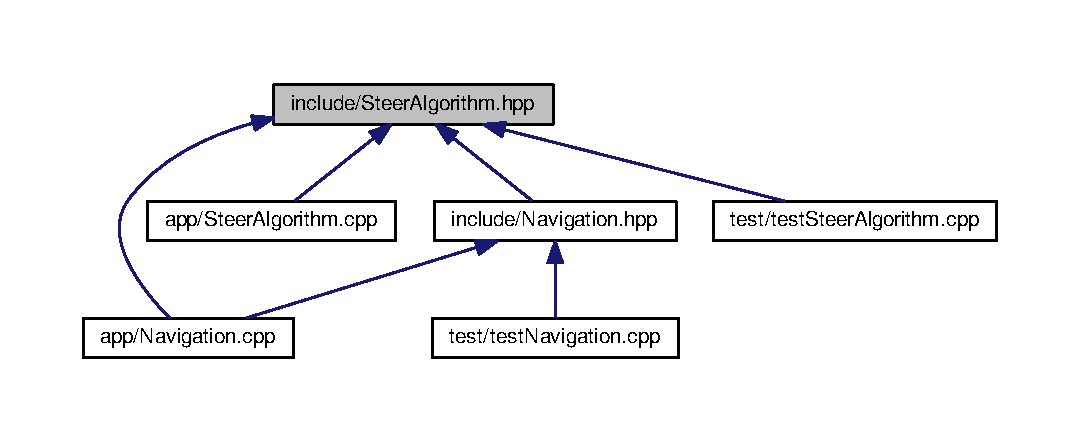
\includegraphics[width=350pt]{_steer_algorithm_8hpp__dep__incl}
\end{center}
\end{figure}
\subsection*{Classes}
\begin{DoxyCompactItemize}
\item 
class \hyperlink{class_steer_algorithm}{Steer\+Algorithm}
\begin{DoxyCompactList}\small\item\em Class \hyperlink{class_steer_algorithm}{Steer\+Algorithm} contains the methods of the Steering Algorithm. \end{DoxyCompactList}\end{DoxyCompactItemize}


\subsection{Detailed Description}
Mid Term Project. 

\begin{DoxyCopyright}{Copyright}
M\+IT License, Copyright © 2019 Raj Shinde
\end{DoxyCopyright}
\begin{DoxyAuthor}{Author}
Sprint-\/1 Raj Shinde-\/ driver and Prasheel Renkuntla-\/ navigator 

Sprint-\/2 Prasheel Renkuntla-\/ driver and Raj Shinde-\/ navigator 
\end{DoxyAuthor}
\begin{DoxyDate}{Date}
10/10/2019 
\end{DoxyDate}
\begin{DoxyVersion}{Version}
6.\+0 
\end{DoxyVersion}
\hypertarget{_steer_algorithm_8hpp_Ackermann}{}\subsection{Steering Control Header file}\label{_steer_algorithm_8hpp_Ackermann}

\hypertarget{test_8cpp}{}\section{test/test.cpp File Reference}
\label{test_8cpp}\index{test/test.\+cpp@{test/test.\+cpp}}


Mid Term Project.  


{\ttfamily \#include $<$gtest/gtest.\+h$>$}\\*
{\ttfamily \#include $<$cstdlib$>$}\\*
{\ttfamily \#include $<$memory$>$}\\*
{\ttfamily \#include \char`\"{}Navigation.\+hpp\char`\"{}}\\*
{\ttfamily \#include \char`\"{}Steer\+Algorithm.\+hpp\char`\"{}}\\*
Include dependency graph for test.\+cpp\+:
\nopagebreak
\begin{figure}[H]
\begin{center}
\leavevmode
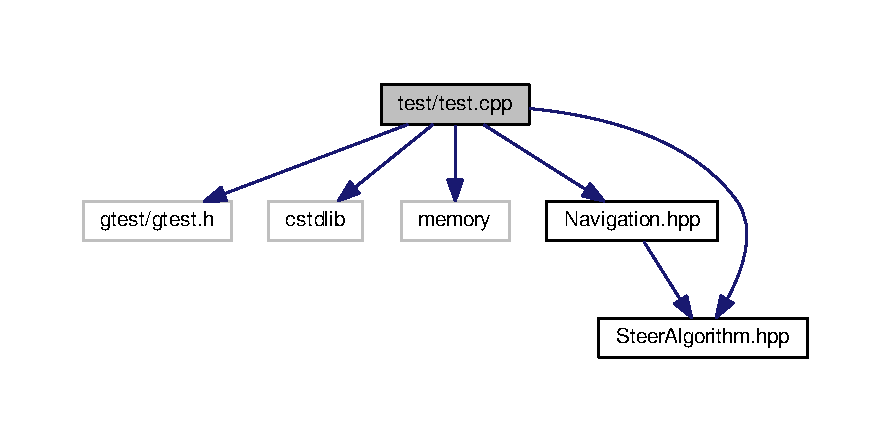
\includegraphics[width=350pt]{test_8cpp__incl}
\end{center}
\end{figure}
\subsection*{Functions}
\begin{DoxyCompactItemize}
\item 
\hyperlink{test_8cpp_a093604a7433c91e9a41a6c486ff843b3}{T\+E\+ST} (\hyperlink{class_navigation}{Navigation}, test\+Set\+Pid)\hypertarget{test_8cpp_a093604a7433c91e9a41a6c486ff843b3}{}\label{test_8cpp_a093604a7433c91e9a41a6c486ff843b3}

\begin{DoxyCompactList}\small\item\em Test to check the set functions for kp\+\_\+,ki\+\_\+ and kd\+\_\+. \end{DoxyCompactList}\item 
\hyperlink{test_8cpp_a5c632ae16e5ba30ae35d75900430e15a}{T\+E\+ST} (\hyperlink{class_navigation}{Navigation}, test\+Get\+Pid)\hypertarget{test_8cpp_a5c632ae16e5ba30ae35d75900430e15a}{}\label{test_8cpp_a5c632ae16e5ba30ae35d75900430e15a}

\begin{DoxyCompactList}\small\item\em Test to check that values of kp\+\_\+,ki\+\_\+ and kd\+\_\+ are below 1 or not. \end{DoxyCompactList}\item 
\hyperlink{test_8cpp_a87664aeb63270d8e6408aa77a3db7d61}{T\+E\+ST} (\hyperlink{class_navigation}{Navigation}, test\+Velocity)\hypertarget{test_8cpp_a87664aeb63270d8e6408aa77a3db7d61}{}\label{test_8cpp_a87664aeb63270d8e6408aa77a3db7d61}

\begin{DoxyCompactList}\small\item\em Test to check the output of P\+ID Controller in the first cycle is within the set bound. \end{DoxyCompactList}\item 
\hyperlink{test_8cpp_a302ee9fe0ef08a6beaea103c911981ff}{T\+E\+ST} (\hyperlink{class_steer_algorithm}{Steer\+Algorithm}, test\+Corr\+Radius)\hypertarget{test_8cpp_a302ee9fe0ef08a6beaea103c911981ff}{}\label{test_8cpp_a302ee9fe0ef08a6beaea103c911981ff}

\begin{DoxyCompactList}\small\item\em Tests to check that the set functions works and the value of corr\+Radius in below setlimit. \end{DoxyCompactList}\item 
\hyperlink{test_8cpp_ab38a7e56f4e7418febe58d9daf9e4b58}{T\+E\+ST} (\hyperlink{class_steer_algorithm}{Steer\+Algorithm}, testwheel)\hypertarget{test_8cpp_ab38a7e56f4e7418febe58d9daf9e4b58}{}\label{test_8cpp_ab38a7e56f4e7418febe58d9daf9e4b58}

\begin{DoxyCompactList}\small\item\em Tests to check if the wheel angles get resetted and the Ackeermann kinematic model is is properly implemented. \end{DoxyCompactList}\item 
\hyperlink{test_8cpp_a2e8c38dec883b8cfc46adb1e0cedb000}{T\+E\+ST} (\hyperlink{class_steer_algorithm}{Steer\+Algorithm}, test\+Calculations)\hypertarget{test_8cpp_a2e8c38dec883b8cfc46adb1e0cedb000}{}\label{test_8cpp_a2e8c38dec883b8cfc46adb1e0cedb000}

\begin{DoxyCompactList}\small\item\em Test to check the functions arclength and turn\+Time provide right length and time values. \end{DoxyCompactList}\end{DoxyCompactItemize}


\subsection{Detailed Description}
Mid Term Project. 

\begin{DoxyCopyright}{Copyright}
M\+IT License, Copyright © 2019 Raj Shinde
\end{DoxyCopyright}
\begin{DoxyAuthor}{Author}
Sprint-\/1 Raj Shinde-\/ driver and Prasheel Renkuntla-\/ navigator 

Sprint-\/2 Prasheel Renkuntla-\/ driver and Raj Shinde-\/ navigator 
\end{DoxyAuthor}
\begin{DoxyDate}{Date}
10/10/2019 
\end{DoxyDate}
\begin{DoxyVersion}{Version}
1.\+0 
\end{DoxyVersion}

%--- End generated contents ---

% Index
\backmatter
\newpage
\phantomsection
\clearemptydoublepage
\addcontentsline{toc}{chapter}{Index}
\printindex

\end{document}
